The motivation of the testbeam measurements are both the testing of TJ-Mopopix1 in condition different from the one forseen during the design and the testing the mechanical and the DAQ setup for other tests in future. I recall that TJ-Monopix1 is supposed to be employed for tracking in HEP experiments while our goal was testing the possibility of integrating charge released by more particles on the sensor at ultra high hit rate .
\red{Una frase di disclaimer sul fatto che non siamo riusciti a testare quello che volevamo.}

The measurements have taken place at the Santa Chiara hospital in Pisa, were a new accelerator for reasearch the FLASH-RT strudys have been recently installed. 
The accelerator is an electron linac of energy in 7-9 MeV  e può arrivare fino a 40 Gy/pulse and it is the only almost the one in the world to access many different beam parameters. Altri accelerati per la flash riescono ad arrivare a... ma non hanno un range di aprametri così grande. \red{ricontrolla sulla review, c'era qualcosa che puoi dire. }
This charateristic is faundamental for research in FLASH, both for the clinical (specifica che sarà usato in vitro o su animali) and medical studies and for the medical teqnical arrangment. 
Infatti ci sono sia ancora questioni aperte per quanto riguarda la medicina e il funzionamento in base ai parametri che per il funzionamento di device. 

The typical beam structure of medical beam is reported in figure \ref{fig:}; in medical physics the parameters used to describe the beam with their description is reported in table \ref{tab:}. 
\begin{figure}
   \centering
   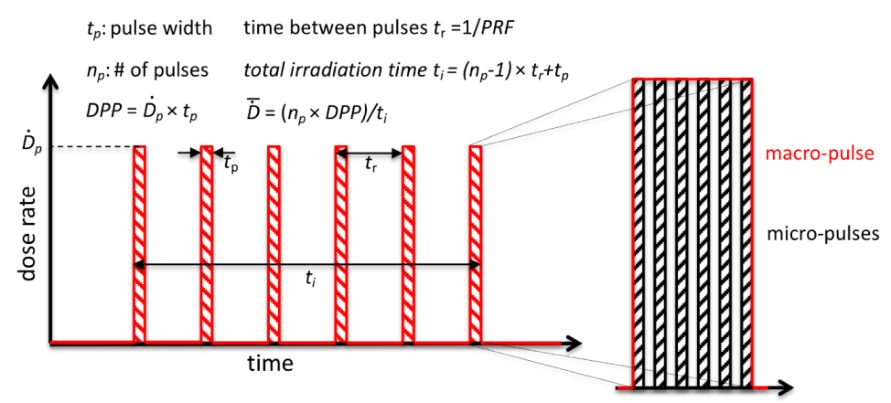
\includegraphics[width=.9\linewidth]{figures/test_beam/beam_structure.pdf}
   \caption{}
   \label{fig:}
\end{figure}

\begin{table}
   \begin{center}
   \begin{tabular}{| c | c | c |}
   \hline
   \\
   \hline
   \hline
Dose rate & $\bar{D}$ & Mean dose rate for a multi-pulse delivery\\
Intra pulse dose rate & $\Dot{\bar{D}}$ & Dose rate in a single pulse \\
Dose per pulse & DDP & Dose in a single pulse \\
Pulse repetition frequency & PRF & Number of pulses delivered per unit of time\\
Pulse width & t$_{p}$ & Duration of a single pulse\\
   \hline
   \end{tabular}
   \caption{}
   \label{tab:}
   \end{center}
\end{table}    

In fisica medica si utilizza la dose, il parametro fondamentale per parametrizzare il danno apportato alle cellule. Una parametrizzazione in rate sarebbe però necessaria per avere un confronto sugli strumenti. 
Per la covnersione si può effettuare un semplice ragionamento ricordando la def di dose, energia assorbita in acqua: 
\ref{disegno del fascio che incide sul fantoccio d'acqua}

Dunque per una determinata sezione del fascio, considerando una massa d'acqua in cui gli elettroni vengono fermati di X0 per Sezione fascio, si ha :


Quindi per avere una conversione di dose in elettroni si usa:
\begin{equation}
   R[Hz/cm^2] = \frac{DPP[Gy]}{1.6 \;10^{10} S[g/cm^2]}
\end{equation}
where S is the stopping power in water, \SI{2.17}{g/cm\squared}
The medium is ordinarily water, since dosimetric protocols are based on measurements in water as reference


Dunque visti gli altissimi rate in gioco, con i tempi morti del nostro chip , non è possibile avere un segnale di singole particelle, perchè in tal caso si satura completamente. 
Ricordiamo che i tempi morti dipendono dal rate e anche dalla posizione del pixel nella matrice, in particolare secondo la priority chain l'ultimo pixel che viene letto è qurllo con tau più lungo. Con un tau medio di 1 us per pixel. 
L'idea è comunque anche se non si riesce a misurare intra pulse e misurare tra i pulse: quindi far sì che la lettura tra l'arrivo di due buch consecutivi. 

Avendo un cut off massimo di hit a 25000 (n of pixel per un flavor), l'idea che si vuole testare è dunque: possibilità di integrare carica sul pixel: due elettroni consecutivi su un pixel ogni quanto arrivano?
Vogliamo sfruttare il analog pile up tra gli eventi, e la linearità del tot. 
   \red{conti}
Devi avere che il tot dell'elettrone (cioè MIP) è maggiore del deltat medio; in questo caso potresti riuscire ad integrare carica.

Purtroppo non è stato possibile effettuare questo test per mancanza di tempo (\red{chiedere a forti}), ma abbiamo effettuato solo un test preliminare, le cui misure sono riportate in sezione. 
   

\section{Apparatus description}
   I parametri che l'acceleratore permette di settare sono: TABELLA
   L'acceleratore è fatto così: ha un tubo di plexiglas (metti una foto) su cui vengono fatti scattereare gli elettroni in modo che all'uscita abbiano una curva di isodose più o meno uniforme. Quindi gli eletrtoni escono con una divergenza.
   \red{metti plot delle curve di isodose e spiega cosa significa}   

   Per effettuare le misure è stato costruito un carrello su cui mettere il DUT, foto del carrello, con la possibilità di regolare la distanza tra dut e bocca del triodo. 

   per schermare gli elttroni dei collimatori sono stati costruiti: uno con posizione fissa da mettere vicino al triodo e uno da mettere lontano con posizione spostabile in modo da illuminare solo una parte del DUT. 
   Collimatori di alluminio spessi 3 cm con fori da 1mm. Il collimatore vicino al triodo ha la funzione di fare una sorgente puntiforme se ci si mette lontano dal fascio, in modo da avere possibilità di diminuire il rate a piacimento come 1/l2.
   Questo ovviamente è reso possibile dal fatto che il fascio ha una divergenza superiore a 1/20, non collimato. 
   \begin{figure}[h!]
      \centering
      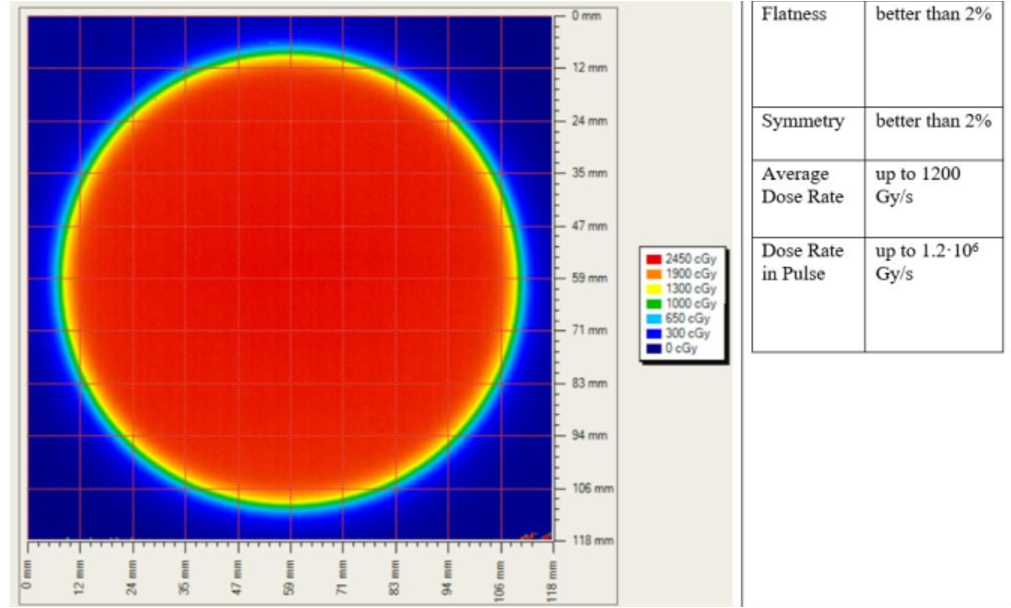
\includegraphics[width=.49\linewidth]{figures/test_beam/dose_profile_10cm.pdf}
      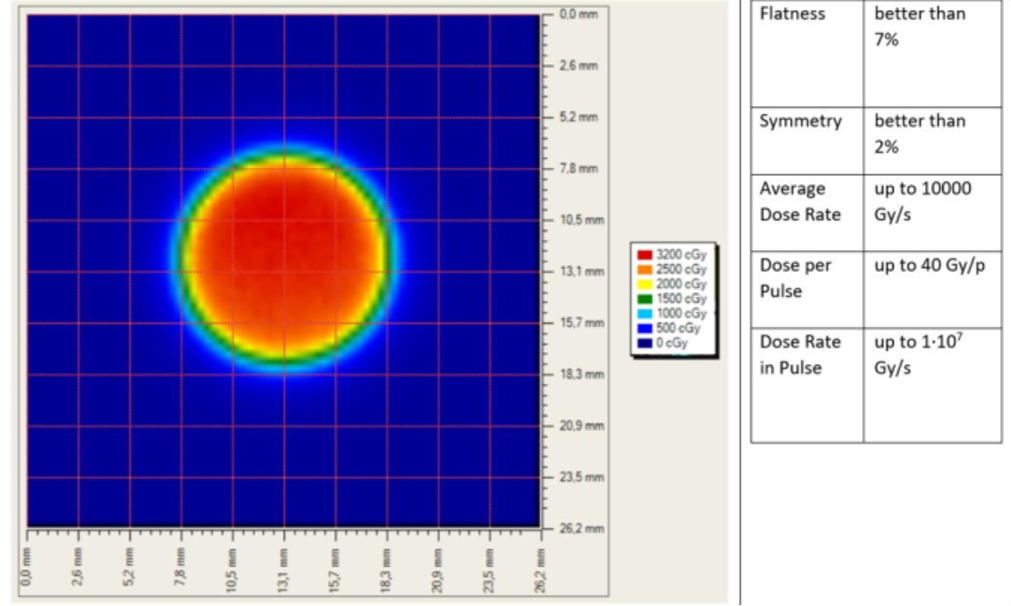
\includegraphics[width=.49\linewidth]{figures/test_beam/dose_profile_1cm.pdf}
      \caption{}
      \label{fig:dose_profile}
   \end{figure}     


\section{Measurements}
   We have used the PMOS flavor (1) with the standard configuration with the idea of starting by testing the setup: we have biased the PWELL and PSUB at -\SI{6}{V} and with the default FE parameters reported in table \ref{tab:FE_default}.
   Initially we have used both the collimators and injected smaller dose pulses and only after we have removed the collimators and increased the DDP. 
   During all the acquisitions we have used pulses with t$_p$ of \SI{4}{\um} and with the smallest PRF settable, which is \SI{1}{Hz}, in order to start in the most conservative working point exluding the digital pile up from different pulses. Indeed the readout time for each pixel is $\sim$\SI{1}{\us}, then even if the whole matrix turns on, the readout time corresponds to \SI{25}{ms}. 

   We encountered a photon background higher than expected: photons are mainly produced via Bremsstrahlung during the transition of electrons through the alluminium collimators.
   \red{qualche numero in più sulla perdita di energia per rad, e magari plot della simulazione}.

   Since the long dead time of the matrix, each pixel cannot fire more than a time for each pulses. 
   Since the readout strarts $\sim$\SI{50}{clk} counts after the first TE of the pixel arrived, we could resolve the pulse in two different part. 
   The hit which arrives and which goes under the thre. during the first 50 clk counts are classified in the first sub-pulse, while the hits which arrives during the freeze are in the second. In the second pulse there are also the hits arrived in the first but with a longer tot (scendono sotto soglia quando ormai è partito il freeze). 
   During the freeze possono arrivare hit, su pixel vuoti. Questi verranno letti dopo. 
   Obviously since the readout of the fist subpulse finished much later the bunch finished, each pixel can be store only one hit. 
   This constitute our saturation, since we can't read more tha 25 000 hits per bunch. 
   Actually this is not completely true, since the firsts pixels in the priority chain, which can be read before the bunch finished, can be hit again and can store a new hit. 
   An example of the two subpulse is shown in figure \ref{fig:}. with a map of the tot of the hit. 

   When we have put aside the collimators, the fluence was too high that the whole matrixs turn on in 50 clock counts; then the 2 pulses substructure no more appears. Also the spectrum change from the previous one. 
   It is shown in figure \ref{fig:}.
   Since a MIP should produce e- in the epitaxial layer, it should provide a signal of about \SI{2}{ke-}, so in our condition it shoud have done rollover. 
   In order to compare the spectrum with the one produced by MIP, in laboratory we have done some acquisitions with cosmic rays. 
   To be confident with having selected MIPS from cosmic rays and not noise, we have selected only the events with one more hits per timestamp, which we consider are prevalentemente cluster. Dato il rate dei cosmici e il rate del rumore infatti, le coincidenze casuali per il nosrto tempo di acquisizione sono.. Qualche esempio di traccia di muoni. e n of hit cluster. 
   Un confrontare degli spettri (convertiti in carica). 


   \begin{figure}
      \centering
      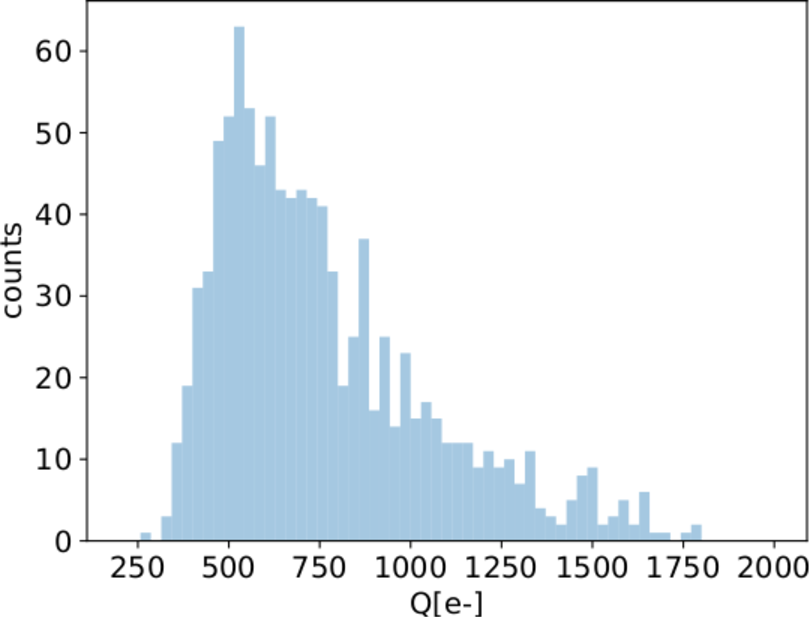
\includegraphics[width=.49\linewidth]{figures/test_beam/Q1_17_11.pdf}
      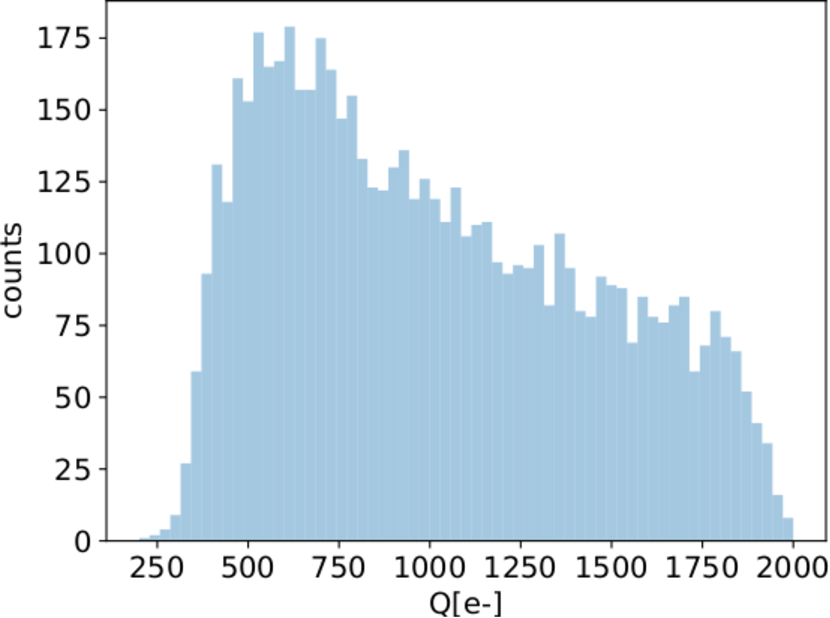
\includegraphics[width=.49\linewidth]{figures/test_beam/Q2_17_11.pdf}\\   
      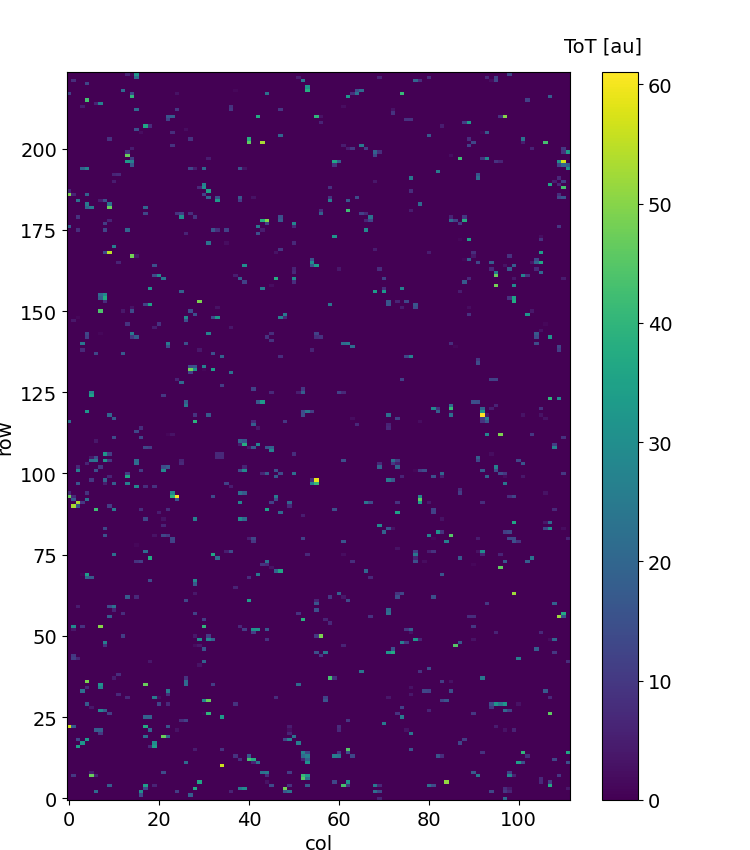
\includegraphics[width=.49\linewidth]{figures/test_beam/tot_mapq1_17-11.png}
      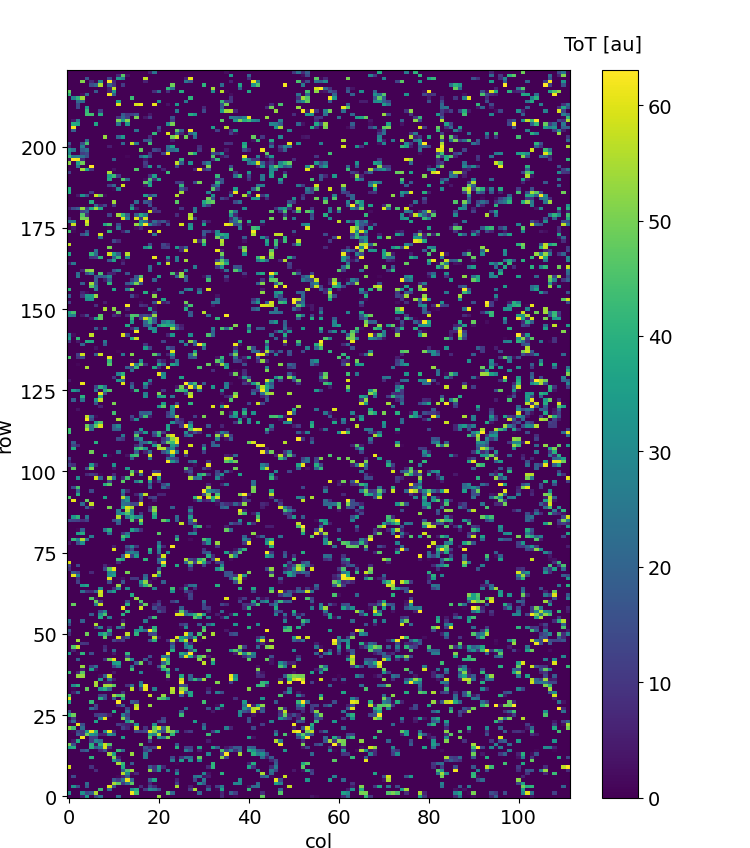
\includegraphics[width=.49\linewidth]{figures/test_beam/tot_mapq2_17-11.png} 
      \caption{Acquisition with both the collimators at DDP=\SI{0.04}{Gy}}
      \label{fig:}
   \end{figure}


   \begin{figure}
      \centering
      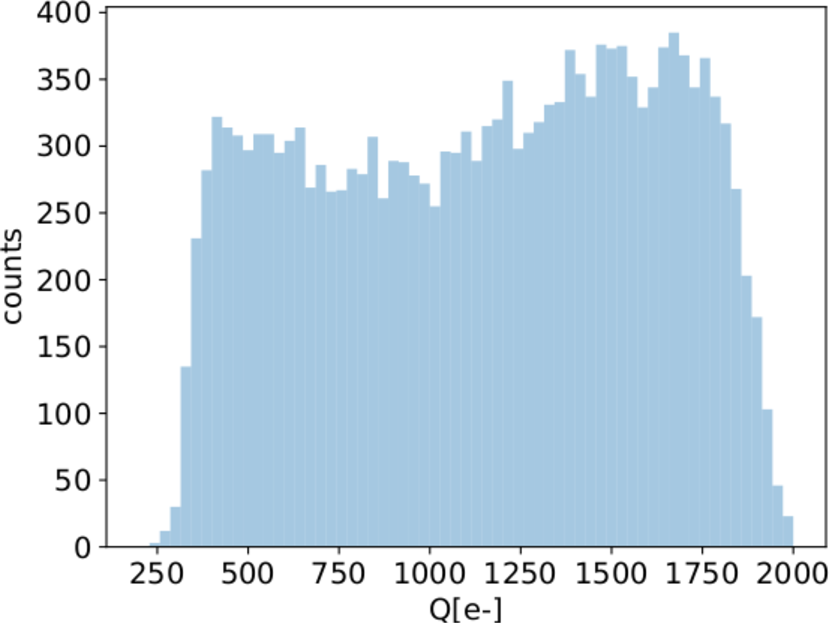
\includegraphics[width=.7\linewidth]{figures/test_beam/Qe_17_32.pdf}
      \caption{Acquisition without any collimator at DDP=\SI{0.04}{Gy}}
      \label{fig:}
   \end{figure}



   \begin{figure}
      \centering
      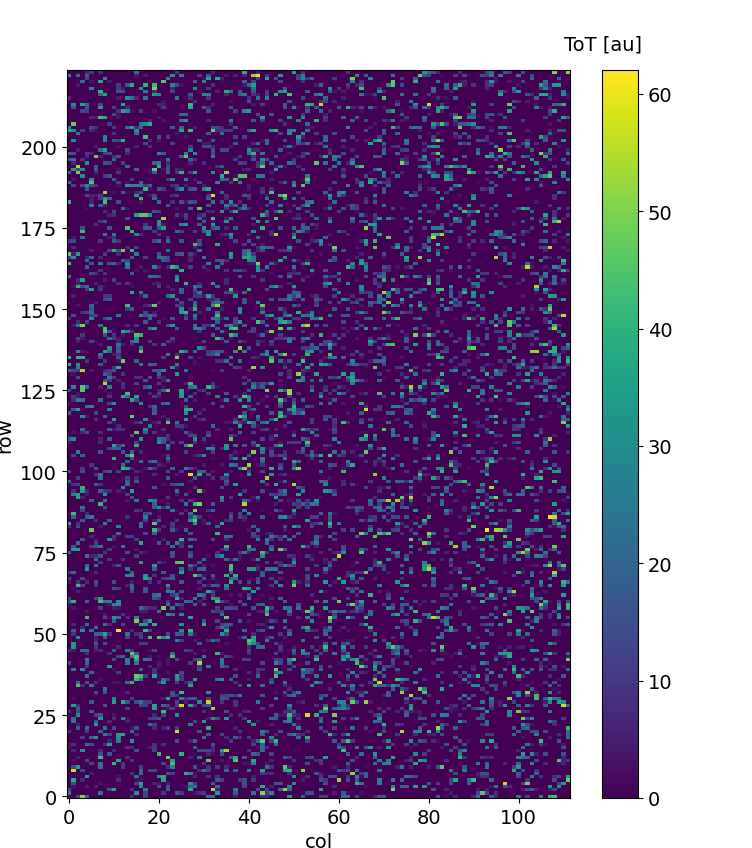
\includegraphics[width=.49\linewidth]{figures/test_beam/tot_mapq1_15-57.png}
      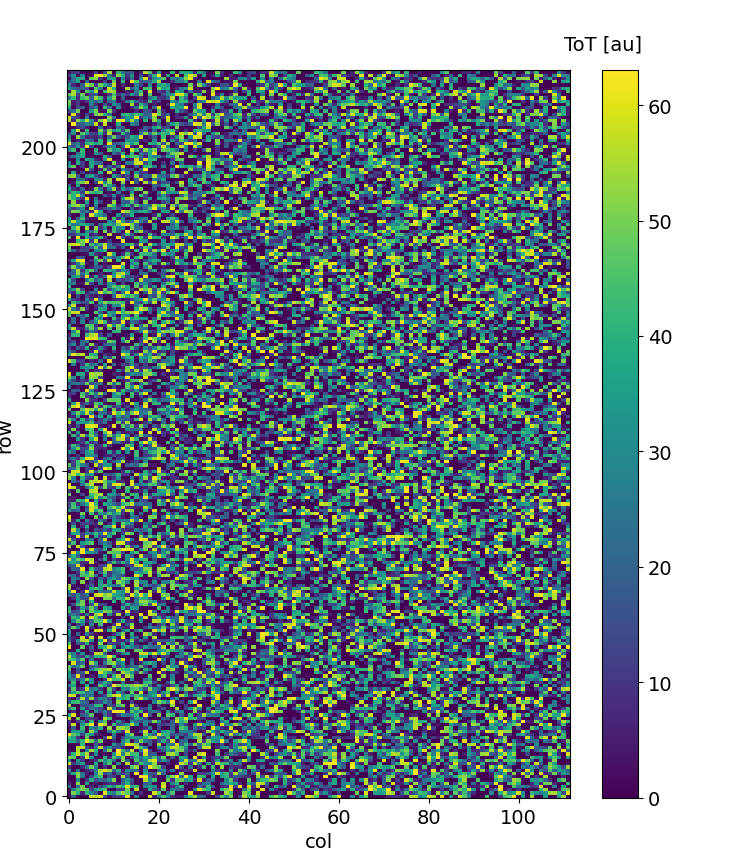
\includegraphics[width=.49\linewidth]{figures/test_beam/tot_mapq2_15-57.png}  
      \caption{}
      \label{fig:}
   \end{figure}

   \begin{table}
      \begin{center}
      \begin{tabular}{| c | c | c |}
      \hline
      DDP & Hits per pulse &    \\
      \hline
      \hline



      \end{tabular}
      \caption{}
      \label{tab:}
      \end{center}
   \end{table}   


